\clearpage

\lehead[]{\sf\hspace*{-2.00cm}\textcolor{white}{\colorbox{lightblue}{\parbox[c][0.70cm][b]{1.60cm}{
\makebox[1.60cm][r]{\thechapter}\\ \makebox[1.60cm][r]{ÜBUNG}}}}\hspace{0.17cm}\textcolor{lightblue}{\chaptertitle}}
\rohead[]{\textcolor{lightblue}{\chaptertitle}\sf\hspace*{0.17cm}\textcolor{white}{\colorbox{lightblue}{\parbox[c][0.70cm][b]{1.60cm}{\thechapter\\
ÜBUNG}}}\hspace{-2.00cm}}
%\chead[]{}
\rehead[]{\textcolor{lightblue}{AvHG, Inf, My}}
\lohead[]{\textcolor{lightblue}{AvHG, Inf, My}}

\section{Vererbung -- Übungen}

\subsection{Aufgabe 1: Übung zur Datenkapselung}

Das UML-Klassendiagramm zeigt mehrere Klassen, die sich in zwei verschiedenen
Packages befinden. Vereinfacht kann man sagen, dass ein Package aus allen
Dateien in einem Verzeichnis besteht. Wenn man auf Klassen aus einem fremden
Package zugreifen möchte, muss man die Klassen mit Hilfe einer \verb|import|-
Anweisung in die Datei einbinden.

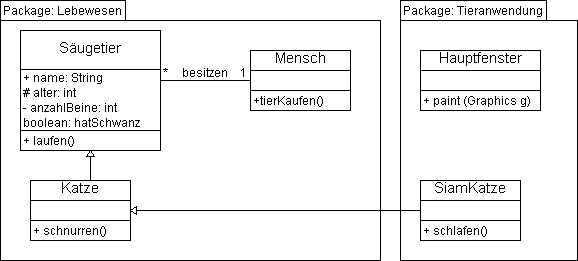
\includegraphics[width=1.0\textwidth]{./inf/SEKII/16_Java_Vererbung/Aufgabe1.png}

Auf welche der Variablen aus der Klasse Säugetier kann man von den anderen
Klassen aus zugreifen?

\bgroup
\def\arraystretch{1.2}
\begin{tabular}{|l|p{30mm}|p{30mm}|p{30mm}|p{30mm}|}
\hline
\textbf{Variable} &
\textbf{Methode \lstinline|schnurren()|\linebreak für ein Katzen-Objekt} &
\textbf{Methode \lstinline|tierKaufen()|\linebreak für ein Mensch-Objekt} &
\textbf{Methode \linebreak \lstinline|paint(g)|\linebreak für ein Haupt\-fen\-ster-Objekt} & 
\textbf{Methode \lstinline|schlafen()|\linebreak für ein
SiamKatze-Objekt} \\
\hline \verb|name| & & & & \\ \hline
\verb|alter| & & & & \\ \hline
\verb|anzahlBeine| & & & & \\ \hline
\verb|hatSchwanz| & & & & \\ \hline
\end{tabular}
\egroup


\subsection{Aufgabe 2: Leseübung}

Es existiert eine Klasse Tier, die folgendermaßen aussieht:

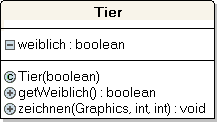
\includegraphics[width=0.3\textwidth]{./inf/SEKII/16_Java_Vererbung/Aufgabe2.png}

Von der Klasse \myClass{Tier} wird eine Klasse \myClass{Hund} abgeleitet. Fülle
die Lücken im Code geeignet aus:

\begin{lstlisting}
public class ____________________________________ {











    public void zeichnen (Graphics g, int x, int y) {æ
        // Nur männliche Hunde sollen gezeichnet werden. Weibliche Hunde
        // verstecken sich. Rufe die Methode zeichnen aus der Superklasse
        // Tier auf, wenn der Hund männlich ist.
æ



    }
}
\end{lstlisting}

\subsubsection{Fragen}

\begin{compactenum}[a)]
\item Wieso gibt es in der überschriebenen Methode \verb|zeichnen(...)| eine
Fehlermeldung, wenn man auf die Variable \verb|weiblich| zugreift?

\item Wieso gibt der Compiler eine Fehlermeldung aus, wenn in der Klasse
\myClass{Hund} kein Konstruktor steht? Schreibe zur Beantwortung der Frage den
Konstruktor auf, den das System automatisch erzeugt.

\item Füge in die Klasse \myClass{Hund} einen Konstruktor ein, der als Parameter
einen boolschen Wert erhält. Der boolsche Wert gibt an, ob der Hund weiblich ist
oder nicht. Dies ist derselbe Konstruktor wie ihn die Superklasse \myClass{Tier}
besitzt.

\item Schreibe zusätzlich einen parameterlosen Konstruktor für die Klasse
\myClass{Hund}, der immer männliche Hunde erzeugt.
\end{compactenum}


\subsection{Aufgabe 3: Zwei spezielle Lampen}

\begin{compactenum}[a)]
\item Verändere die Sichtbarkeit der Attribute in der Klasse \myClass{Lampe}
(du findest die Datei \myFile{Lampe.java} im Kurs-Repository im Ordner
\myFile{16\_Java\_Vererbung}) von \verb|private| nach \verb|protected|.
Ansonsten bleibt die Klasse \myClass{Lampe} unverändert.

\begin{minipage}{0.5\textwidth}
\begin{lstlisting}
public class Lampe {
    protected Color farbe;
    protected boolean isAn = false;
    protected int xPos, yPos;
    protected static final int BREITE = 50;

    ...
}
\end{lstlisting}
\end{minipage}
\hfill
\begin{minipage}{0.4\textwidth}
\textbf{\lstinline|protected|}:\\ Außerhalb des eigenen Packages Zugriff nur für
abgeleitete Klassen.
\end{minipage}

\item In einem neuen Package (nicht das, in welchem die Klasse \myClass{Lampe}
bereits existiert!) sollen zwei spezielle Lampentypen programmiert werden, die
von der Klasse \myClass{Lampe} abgeleitet werden:

\begin{compactenum}[1.]
\item die \myClass{QuadratLampe}, die statt eines runden ein quadratisches Licht
anzeigt.
\item die \myClass{RahmenLampe}, die um den Lichtkreis einen schwarzen Rand
zeichnet.
\end{compactenum}

Welche Attribute und Methoden benötigen die abgeleiteten Klassen?

\item Erstelle im gleichen Package eine Klasse für das Anwendungsprogramm.
Erzeuge im Anwendungsprogramm je ein Objekt der drei Lampen-Klassen, und lass
jede Lampe blinken.

\item Eine Variable der Superklasse \myClass{Lampe} kann auch Objekte
abgeleiteter Klassen speichern.

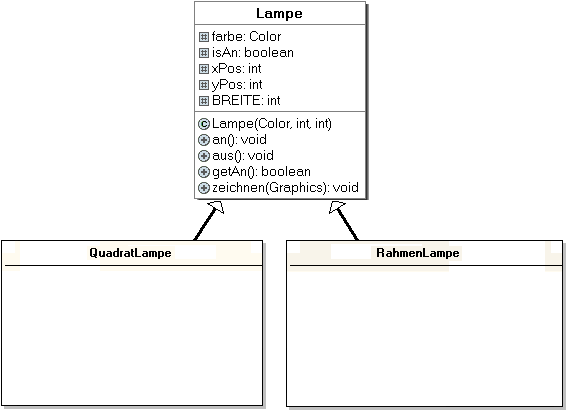
\includegraphics[width=0.8\textwidth]{./inf/SEKII/16_Java_Vererbung/Aufgabe3.png}

Erzeuge im Anwendungsprogramm eine weitere Variable vom Typ der Superklasse
\myClass{Lampe}. Weise dieser Variable im Konstruktor des Anwendungsfensters
über eine Zufallszahl ein Objekt von einem der drei Lampen-Typen zu (0
$\rightarrow$ \myClass{Lampe}, 1 $\rightarrow$ \myClass{QuadratLampe}, 2
$\rightarrow$ \myClass{RahmenLampe}). Zeichne auch diese Lampe im
Anwendungsfenster und lass sie blinken.
\end{compactenum}


\subsection{Aufgabe 4: Drachen}

\begin{compactenum}[a)]
\begin{minipage}{0.6\textwidth}
\item Programmiere eine Klasse \myClass{Drachen} (siehe Abbildung). Alle
Attribute der Klasse \myClass{Drachen} sollen vor dem Zugriff von außen
(d.h.\ vom Anwendungsfenster aus) geschützt sein. Alle Methoden sind öffentlich
und dürfen vom Anwendungsfenster aus benutzt werden.

Im Konstruktor der Klasse werden die x-Position, die y-Position
(linke obere Ecke: in der Zeichnung mit einem Kreuz markiert) und
die Farbe des Drachen als Parameter übergeben.

Der Drachen besitzt eine Methode \verb|zeichnen()|, die den Drachen
mit der gewählten Farbe an der eingestellten Position malt. Dazu
werden zwei ausgefüllte Dreiecke gezeichnet. Ein Kästchen in der
Abbildung soll einer Breite von zehn Pixeln entsprechen.

Erzeuge im Anwendungsfenster zwei verschiedene Objekte der
Klasse Drachen.
\end{minipage}
\hfill
\begin{minipage}{0.3\textwidth}
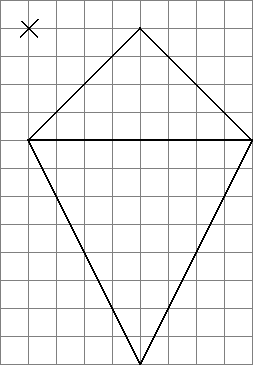
\includegraphics[width=0.8\textwidth]{./inf/SEKII/16_Java_Vererbung/Aufgabe4a.png}
\end{minipage}

\begin{minipage}{0.6\textwidth}
\item Programmiere in einem anderen Package eine Klasse
\myClass{GesichtDrachen}, die sich von der Klasse \myClass{Drachen} ableitet
(siehe Abbildung). Überschreibe die Methode \verb|zeichnen()| und ergänze den
Drachen um zwei blaue Augen und einen roten Mund. Erweitere die Methode so,
dass du den Code zum Zeichnen des Drachen nicht noch einmal neu
programmieren musst.

Erstelle im gleichen Package auch eine Anwendungsklasse und erzeuge im
Anwendungsfenster ein oder mehrere Objekte der Klasse \myClass{GesichtDrachen}.
\end{minipage}
\hfill
\begin{minipage}{0.3\textwidth}
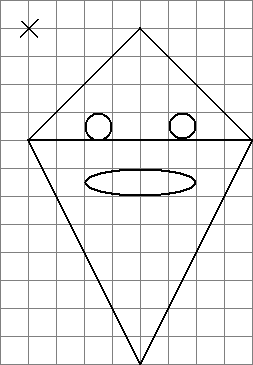
\includegraphics[width=0.8\textwidth]{./inf/SEKII/16_Java_Vererbung/Aufgabe4b.png}
\end{minipage}

\begin{minipage}{0.6\textwidth}
\item Im selben Package sollst du nun auch noch eine Klasse
\myClass{SchwanzDrachen} programmieren , die sich von der Klasse
\myClass{GesichtDrachen} ableitet (siehe Abbildung). Der Konstruktor der Klasse
\myClass{Drachen} soll um einen Parameter erweitert werden, der die Farbe für
den Schwanz des Drachen angibt. Überschreibe die Methode \verb|zeichnen()| und
hänge unten an den Drachen drei farbige Kreise an. Erweitere die Methode
\verb|zeichnen()| so, dass du den Code zum Zeichnen des GesichtDrachen nicht
noch einmal neu programmieren musst.

Erzeuge im Anwendungsfenster ein oder mehrere Objekte der Klasse
\myClass{SchwanzDrachen}.
\end{minipage}
\hfill
\begin{minipage}{0.3\textwidth}
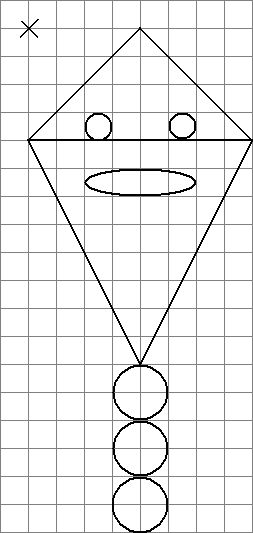
\includegraphics[width=0.8\textwidth]{./inf/SEKII/16_Java_Vererbung/Aufgabe4c.png}
\end{minipage}
\end{compactenum}


\subsection{Aufgabe 5: Schiffe}

\begin{compactenum}[a)]

\item Erzeuge ein Anwendungsfenster mit einem blauen Hintergrund. Das
Anwendungsfenster soll eine Breite und Höhe von je 500 Pixel besitzen. Füge in
das Anwendungsfenster ein Objekt der Klasse \myClass{Timer} ein und stelle eine
Wiederholungsrate von 20 Millisekunden ein.

\begin{minipage}{0.6\textwidth}
\item Programmiere in einem anderen Package eine Klasse \myClass{Schiff}. Alle
Attribute der Klasse \myClass{Schiff} sollen vor dem Zugriff von außen (d.h.
vom Anwendungsfenster aus) geschützt sein. Alle Methoden sind öffentlich und
dürfen vom Anwendungsfenster aus benutzt werden.

Der Klasse \myClass{Schiff} wird im Konstruktor eine Farbe, die anfängliche y-
Position und ein Wert für die Geschwindigkeit (\verb|speed|) übergeben. Die
anfängliche x-Position wird automatisch auf 0 gesetzt.

Programmiere eine Methode \verb|bewegen()|, die das Schiff jeweils um
den in der Variablen \verb|speed| stehenden Wert nach rechts verschiebt.
Sobald die x-Position größer als 500 ist, wird das Schiff 110 Pixel vor
den linken Rand gesetzt, damit es wieder langsam in das Bild
hineingleitet.
\end{minipage}
\hfill
\begin{minipage}{0.3\textwidth}
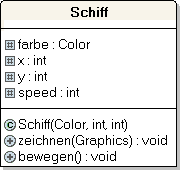
\includegraphics[width=0.8\textwidth]{./inf/SEKII/16_Java_Vererbung/Aufgabe5b1.png}
\end{minipage}

\begin{minipage}{0.5\textwidth}
Schreibe eine Methode \verb|zeichnen()|, die das Schiff an
seiner aktuellen Position in der gewählten Farbe zeichnet.
Das Schiff wird mit einem ausgefüllten Rechteck und zwei
angrenzenden ausgefüllten Dreiecken gezeichnet. Die
Position, die durch die x- und die y-Koordinate beschrieben
wird, ist in der Abbildung durch ein Kreuz markiert. Ein
Kästchen soll eine Breite von 10 Pixel besitzen.
\end{minipage}
\hfill
\begin{minipage}{0.4\textwidth}
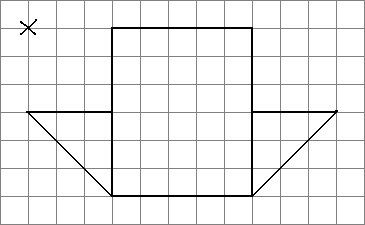
\includegraphics[width=1.0\textwidth]{./inf/SEKII/16_Java_Vererbung/Aufgabe5b2.png}
\end{minipage}

\item Erzeuge im Anwendungsfenster ein oranges (\verb|Color.ORANGE|) Schiff mit
der y-Position 200 und einer Geschwindigkeit (\verb|speed|) von 2. Erzeuge ein
zweites Schiff mit der Farbe \verb|PINK|, der y-Position 50 und einer
Geschwindigkeit von 3. Rufe für beide Schiffe in der \verb|myPaint()|-Methode
die beiden Methoden \verb|bewegen()| und \verb|zeichnen()| auf.

\item Leite von der Klasse \myClass{Schiff} die Klasse \myClass{FensterSchiff}
ab. Die Klasse \myClass{Fensterschiff} soll im selben Package liegen, wie die
Klasse des Anwendungsfensters. Das Fensterschiff besitzt zusätzlich zwei
Fenster, die als ausgefüllte, gelbe Kreise gezeichnet werden (siehe Abbildung).
Füge diese Erweiterung so ein, dass die Zeichen-Funktionalität der Oberklasse
wieder verwendet wird.

\begin{center}
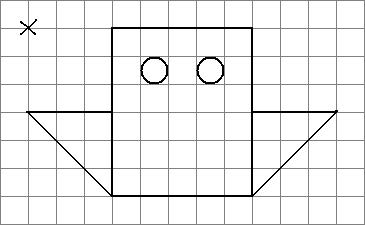
\includegraphics[width=0.4\textwidth]{./inf/SEKII/16_Java_Vererbung/Aufgabe5d.png}
\end{center}

Erzeuge im Anwendungsfenster ein Objekt der Klasse \myClass{FensterSchiff} mit
der Farbe \verb|LIGHT_GRAY|, der y-Position 150 und einer Geschwindigkeit von 4.

\item Zeichne im Anwendungsfenster an der Position (200, 400) ein ausgefülltes
Rechteck mit einer Breite von 110 und einer Höhe von 100 Pixel ein. Das
Rechteck soll die Farbe \verb|LIGHT_GRAY| besitzen. Dieses Rechteck soll einen
Steg darstellen, an dem Schiffe anlegen können.

\item Programmiere eine Klasse \myClass{AnlegeSchiff} (wiederum im selben
Package), die sich von \myClass{FensterSchiff} ableitet. Im
Konstruktor des AnlegeSchiffs wird zusätzlich zu den geerbten Parametern eine
Integer-Variable übergeben, in der die Position des Stegs steht. Wenn das
Schiff mit seiner x-Position auf den Steg trifft, soll es 30 Aufrufe der
Methode bewegen lang stehen bleiben. Danach fährt es mit der alten
Geschwindigkeit weiter. Programmiere diese Erweiterung so, dass die
Bewegungsänderung nicht neu geschrieben werden muss.

Erzeuge im Anwendungsfenster ein AnlegeSchiff mit der Farbe \verb|PINK|, der
y-Position 340, der Geschwindigkeit 2 und der Stegposition 200.
\end{compactenum}


\subsection{Aufgabe 6: Billardkugeln}

Verschiedene Billardkugeln sollen über den Bildschirm rollen. Wenn eine Kugel
an den Rand des Fensters stößt, prallt sie vom Rand ab und bekommt eine neue
Richtung nach dem Gesetz „Einfallwinkel gleich Ausfallwinkel“. Dafür muss die
Kugel die aktuelle Fenstergröße kennen.

\begin{center}
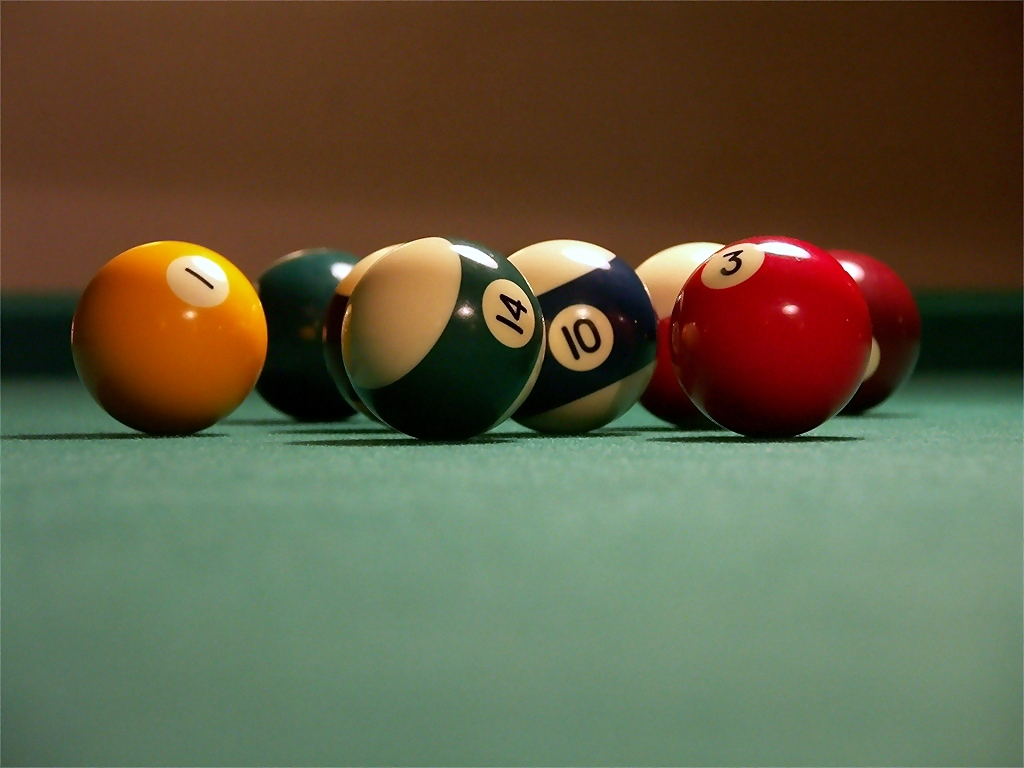
\includegraphics[width=0.4\textwidth]{./inf/SEKII/16_Java_Vererbung/Billiards_balls.jpg}
% http://commons.wikimedia.org/wiki/File:Billiards_balls.jpg
\end{center}

Neben den „einfachen“ Billardkugeln existieren eine Reihe von speziellen Kugeln:

\begin{compactitem}
\item Nummernkugel : Die Kugel zeigt in ihrem Innern eine Nummer an.
\item Pulsierkugel: Die Kugel soll langsam größer und dann wieder kleiner
werden. Das Wachsen und Schrumpfen soll ständig passieren.
\item Reibungskugel : Die Kugel reagiert auf Reibung und wird nach jedem Stoß
gegen die Fensterwand langsamer.
\end{compactitem}

Programmiere zunächst eine „einfache“ Kugel und teste sie aus (siehe dazu den
letzten Abschnitt \glqq Die Billard-Anwendung\grqq ).
Programmiere dann nach und nach die Spezialkugeln und teste sie.


\subsubsection{Entwurf für die Billardkugeln}

\begin{center}
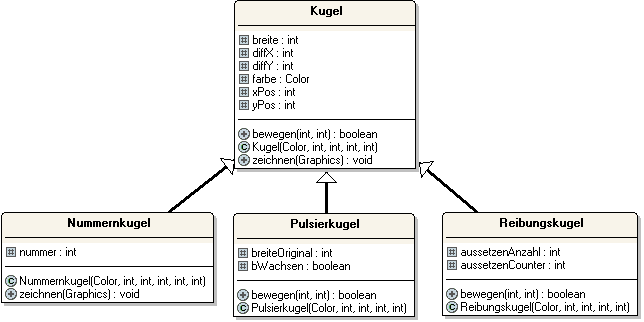
\includegraphics[width=1.0\textwidth]{./inf/SEKII/16_Java_Vererbung/Aufgabe6.png}
\end{center}


\subsubsection{Klasse Kugel}

Die linke obere Ecke einer Kugel wird mit den Integer-Variablen \verb|xPos| und
\verb|yPos| bezeichnet. Die \verb|breite| entspricht dem Durchmesser der Kugel.
Die Geschwindigkeit und die Richtung werden über die Integer-Variablen
\verb|vX| und \verb|vY| ausgedrückt. \verb|vX| gibt die Änderung der
Geschwindigkeit in x-Richtung an, während \verb|vY| die Änderung in
y-Richtung angibt. Beide Werte werden bei jedem Aufruf der Methode
\verb|bewegen()| zu \verb|xPos| bzw. \verb|yPos| dazu addiert. Im Konstruktor
werden die Farbe sowie die Variablen \verb|xPos|, \verb|yPos|, \verb|vX| und
\verb|vY| übergeben. Die \verb|breite| wird automatisch auf 20 Pixel gesetzt
(oder einen anderen geeigneten Wert).

Die Methode \verb|zeichnen()| zeichnet die Kugel an ihrer aktuellen Position.
Die Methode \verb|bewegen()| bewegt die Kugel wie oben beschrieben weiter. Als
Parameter erhält \verb|bewegen()| die Breite und die Höhe des Fenster. Als Hilfe
für die Reibungskugel gibt sie einen boolschen Wert zurück, der angibt, ob die
Kugel gegen die Wand gestoßen ist (\verb|true|) oder nicht (\verb|false|).

\subsubsection{Programmierung des Abprallens vom Rand}

\begin{minipage}{0.15\textwidth}
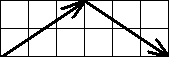
\includegraphics[width=1.0\textwidth]{./inf/SEKII/16_Java_Vererbung/abprallen_oben.png}
\end{minipage}
\hfill
\begin{minipage}{0.2\textwidth}
\begin{tabular}{ll}
\textbf{vorher:}  & vX = \\
                  & vY = \\
                  &      \\
\textbf{nachher:} & vX = \\
                  & vY = \\
                  &      \\
\end{tabular}
\end{minipage}
\hfill
\begin{minipage}{0.2\textwidth}
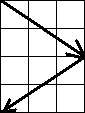
\includegraphics[width=0.4\textwidth]{./inf/SEKII/16_Java_Vererbung/abprallen_seite.png}
\end{minipage}
\begin{minipage}{0.2\textwidth}
\begin{tabular}{ll}
\textbf{vorher:}  & vX = \\
                  & vY = \\
                  &      \\
\textbf{nachher:} & vX = \\
                  & vY = \\
                  &      \\
\end{tabular}
\end{minipage}
\hfill

\subsubsection{Klasse Nummernkugel}

Die Klasse \myClass{Nummernkugel} wird um ein zusätzliches Attribut
\verb|nummer| erweitert, in dem die Zahl steht, die in der Kugel angezeigt
werden soll. Der Konstruktor wird um einen Parameter erweitert, in dem die Zahl
übergeben wird. Die Methode \verb|zeichnen()| wird geeignet überschrieben.


\subsubsection{Klasse Pulsierkugel}

Die Klasse \myClass{Pulsierkugel} besitzt denselben Konstruktor wie die
Oberklasse.

Sie überschreibt die Methode \verb|bewegen()|, und erweitert sie um die Änderung
der Kugelgröße. Die Originalbreite wird in einer Variablen abgespeichert. Die
Kugel wächst zunächst schrittweise um einen Pixel bis sie die Originalbreite um
fünf Pixel überschritten hat. Anschließend schrumpft sie schrittweise um einen
Pixel bis sie die Originalbreite um fünf Pixel unterschritten hat, usw. Eine
boolesche Variable speichert die aktuelle Richtung der Größenänderung (wachsen
oder schrumpfen).


\subsubsection{Klasse Reibungskugel}

Die Klasse \myClass{Reibungskugel} besitzt denselben Konstruktor wie die
Oberklasse und überschreibt die Methode \verb|bewegen()|. Die Verlangsamung
der Bewegung wird programmiert, indem die Kugel bei der Bewegungsänderung
„Aussetzer“ hat. Nach dem ersten Stoß gegen die Wand wird die Position der
Kugel nur noch bei jedem zweiten Aufruf der Methode \verb|bewegen()| tatsächlich
verändert. Nach dem nächsten Stoß wird einmal die Bewegung geändert und dann
zweimal ausgesetzt, nach dem darauf folgenden Stoß wird einmal die Bewegung
geändert und dann dreimal ausgesetzt, usw.

Es gibt eine Variable \verb|aussetzenAnzahl|, die angibt, nach wie viel
\verb|bewegen()|-Aufrufen die Bewegung verändert wird. Zu Anfang ist der Wert 0.
Nach dem ersten Stoß gegen die Wand ist der Wert 1, dann 2 usw.
Die Variable \verb|aussetzenCounter| zählt die Anzahl der
\verb|bewegen()|-Aufrufe bis die \verb|aussetzenAnzahl| überschritten ist und
tatsächlich eine Bewegung ausgeführt wird.


\subsubsection{Die Billard-Anwendung}

Erzeuge in einem anderen Package eine Klasse \myClass{Billard}, die von
\myClass{HJFrame} abgeleitet ist. Das Anwendungsfenster soll eine Breite und
Höhe von je 500 Pixeln und einen grünen Hintergrund haben.

Erzeuge von jeder Kugelart je ein Objekt mit geeigneten Startwerten (gib jeder
Kugel eine eigene Farbe und benutze unterschiedliche Anfangspositionen und
Geschwindigkeiten). Erzeuge im Konstruktor der Anwendungsklasse ein geeignetes
Timer-Objekt um die Billardanwendung zu animieren.
